%%%%%%%%%%%%%%%%%%%%%%%%%%%%%%%%%%%%%%%%%
% Thin Sectioned Essay
% LaTeX Template
% Version 1.0 (3/8/13)
%
% This template has been downloaded from:
% http://www.LaTeXTemplates.com
%
% Original Author:
% Nicolas Diaz (nsdiaz@uc.cl) with extensive modifications by:
% Vel (vel@latextemplates.com)
%
% License:
% CC BY-NC-SA 3.0 (http://creativecommons.org/licenses/by-nc-sa/3.0/)
%
%%%%%%%%%%%%%%%%%%%%%%%%%%%%%%%%%%%%%%%%%

%----------------------------------------------------------------------------------------
%	PACKAGES AND OTHER DOCUMENT CONFIGURATIONS
%----------------------------------------------------------------------------------------

\documentclass[a4paper, 11pt]{article} % Font size (can be 10pt, 11pt or 12pt) and paper size (remove a4paper for US letter paper)
\usepackage{listings}   
\usepackage{amsmath}
\usepackage{wrapfig} % Allows in-line images
\usepackage{graphicx}
\usepackage{mathpazo} % Use the Palatino font
\usepackage[T1]{fontenc} % Required for accented characters
\usepackage{floatrow}
\usepackage{lmodern}
\usepackage{graphicx}
\usepackage{amsthm}
\usepackage{float}
\newtheorem*{theorem*}{Theorem}
\newtheorem*{corollary*}{Corollary}
\usepackage{lingmacros}
\linespread{1.05} % Change line spacing here, Palatino benefits from a slight increase by default
\newtheorem{theorem}{Theorem}

\makeatletter
\renewcommand\@biblabel[1]{\textbf{#1.}} % Change the square brackets for each bibliography item from '[1]' to '1.'
\renewcommand{\@listI}{\itemsep=0pt} % Reduce the space between items in the itemize and enumerate environments and the bibliography

\renewcommand{\maketitle}{ % Customize the title - do not edit title and author name here, see the TITLE block below
\begin{flushright} % Right align
{\LARGE\@title} % Increase the font size of the title

\vspace{50pt} % Some vertical space between the title and author name

{\large\@author} % Author name
\\\@date % Date

\vspace{40pt} % Some vertical space between the author block and abstract
\end{flushright}
}

%----------------------------------------------------------------------------------------
%	TITLE
%----------------------------------------------------------------------------------------

\title{\textbf{The Relationship Between\\
Empirical Process and Gaussian Process: An Example in Kolmogrov-Smirov Test}\\ % Title
Stochostic Process: Final Project} % Subtitle

\author{\textsc{Chi-Ning,Chou} % Author
\\{\textit{PROFESSOR RAOUL NORMAND }}} % Institution

\date{\today} % Date

%----------------------------------------------------------------------------------------

\begin{document}

\maketitle % Print the title section

%----------------------------------------------------------------------------------------
%	ABSTRACT AND KEYWORDS
%----------------------------------------------------------------------------------------

%\renewcommand{\abstractname}{Summary} % Uncomment to change the name of the abstract to something else

\begin{abstract}
Kolmogrov-Smirov test is a famous non-parametric goodness of fitting test. The Kolmogrov statistics: $D_n = \sup_{x\in \mathcal{R}}|\hat{F}_n(x)-F(x)|$ is the central idea in this statistical test. $D_n$ is a {\it distribution-free} statistics. The convergence of $D_n$ provides us a way to see that whether a source is sampled from the guessing distribution. Moreover, since the probability distribution of $D_n$ will converge to that of a Brownian Bridge, the confidence interval can be calculated.

A distribution-free statistics, the Kolmogrov statistics, of empirical distribution converging to the Brownian Bridge is so amazing that we further dig into the relationship between empirical process and Gaussian process. Looking forward to find some interesting behaviour among them.
\end{abstract}

\hspace*{5,6mm}\textit{Keywords:} Kolmogrov-Smirov test, Empirical Process, Brownian Bridge, Gaussian Process % Keywords

\vspace{30pt} % Some vertical space between the abstract and first section

%----------------------------------------------------------------------------------------
%	ESSAY BODY
%----------------------------------------------------------------------------------------

\tableofcontents
\setcounter{tocdepth}{1}

\section{Kolmogrov-Smirov Test}
\subsection{Empirical Distribution}
\paragraph{}
As observers, all we can see from a random experiment is the sampling results from an underlying distribution (if there exists one). In almost every case, we don't know the true probability distribution behind it. What we want to do is to make inferences about the underlying distribution.

As long as we only have the samples, it's intuitively to make a histogram and observe the structure. Furthermore, we can consider the {\it empirical distribution function}
$$\hat{F}_n(x):=\frac{1}{n}\sum^{n}_{i=1}{\bf I}_{\{X_i\leq x\}}$$

where $X_1, X_2, ..., X_n$ are i.i.d. sample from a cumulative distribution function $F$. And ${\bf I}$ is the indicator function.

\paragraph{}
The intuition is that we record the number of samples from the small to large and draw a cumulative function.

The empirical distribution function has some nice properties such as point-wise convergence to the underlying distribution: $\hat{F}_n(z)\xrightarrow{P}F(z)$. The result is followed from the observation that the distribution of $n\hat{F}_n(z)$ for some $z\in\mathcal{R}$ is the same as $binomial(n, F(z))$. This observation can be easily seen in figure 1.
\begin{figure}[h]
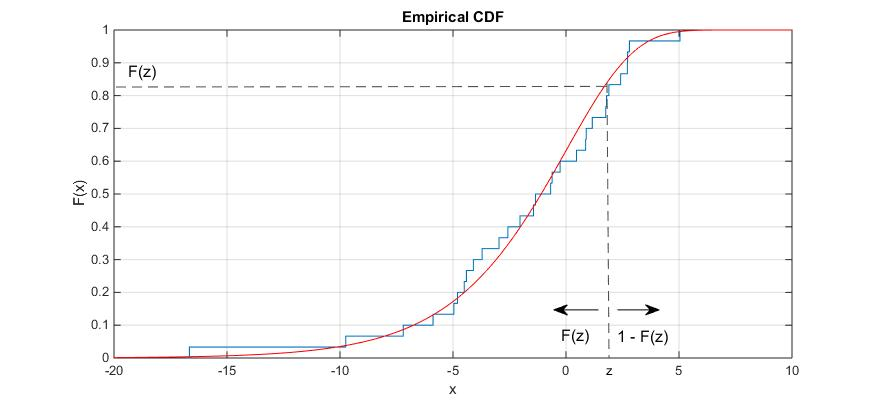
\includegraphics[scale=0.4]{empiricaldistribution_1.jpg}
\caption{Empirical distribution and its point-wise convergence property.}
\end{figure}

Now we have the point-wise convergence of empirical distribution and the corresponding asymptotic rate. Based on this, we can construct confidence interval for point-wise estimation. However, what if we want to estimate the behaviour of two points? Or, the behaviour in an interval?

\subsection{Kolmogrov Statistics}
\paragraph{}
The Kolmogrov statistics is defined on an empirical distribution function $\hat{F}_n$ and a cumulative objective function $F$ as follow:
$$D_n:=\sup_{x\in\mathcal{R}}|\hat{F}_n(x)-F(x)|$$
where $n$ is the number of samples.

We can see that the Kolmogrov statistics $D_n$ is the supremum point-wise distance between the empirical distribution and the target function. The smaller the $D_n$ is we can some how think of that the closer the two distribution are.

As long as we consider the Kolmogrov statistics between the empirical distribution and its underlying distribution, there are some nice convergence behaviours.

\begin{theorem}[Glivenko-Cantelli]
The Kolmogrov statistics will converge to zero as the number of samples grows to infinity. That is,
$$D_n\xrightarrow{P}0$$, as $n\rightarrow\infty$
\end{theorem}

With this theorem, we have the uniform convergence of empirical distribution. Namely, for any $\epsilon > 0$ there exists a $N$ such that for all $n>N$, the underlying distribution will lies in the $\epsilon$-neighborhood of the empirical distribution.

\paragraph{}
In addition, the Kolmogrov statistics has a very important property: {\it distribution-free}. It means that no matter what underlying property is, the behaviour of the Kolmogrov statistics will be the same! Concretely, the distribution will related to the uniform distribution.

\begin{theorem}[Distribution-Free Property]
The distribution of the Kolmogrov statistics $D_n$ is the same for all continuous underlying cumulative distribution.
\end{theorem}

\subsection{Empirical Process Theory}


\section{Brownian Bridge}
\subsection{Gaussian Process}
\subsection{Brownian Bridge}

%------------------------------------------------


\bibliographystyle{plain}
\begin{thebibliography}{9}

\bibitem{CC}
\emph{Crypto Corner},
http://crypto.interactive-maths.com
\bibitem{HG}
\emph{The Hunger Games}, Suzanne Collins. 2008. Scholastic. U.S.
https://sites.google.com/site/the74thhungergamesbyced/download-the-hunger-games-trilogy-e-book-txt-file
\end{thebibliography}

\section*{Appendix}
The code of this project can be found on Github: https://github.com/jerrychou82/MCMC\_Break\_Stream\_Cipher
It's welcome to discuss the code with me!

\end{document}